\selectlanguage{ngerman}%
\frenchspacing%
\begin{ledgroupsized}[r]{120mm}%
\footnotesize%
\pstart%
\noindent\textbf{Überlieferung:}%
\pend%
\end{ledgroupsized}%
\begin{ledgroupsized}[r]{114mm}%
\footnotesize%
\pstart%
\parindent -6mm%
\makebox[6mm][l]{\textit{L}}%
Notiz:
LH XXXVII~4, Bl.\;156.
Ein Zettel (16\;x\;13 cm);
Ränder beschnitten;
Papier\-er\-hal\-tungs\-maß\-nah\-men.
Drei Zeilen auf Bl.\;156\,r\textsuperscript{o}.
Derselbe Träger überliefert zudem N.\;\ref{57037-1} %
sowie eine Notiz über Pyrotechnik (Bl.\;156\,r\textsuperscript{o}) %
und ein Fragment über die Gezeiten %
(Bl.\;156\,r\textsuperscript{o}); beide letzten Texte sollen voraussichtlich in späteren Bänden von \textit{LSB} VIII ediert werden.
\pend%
\end{ledgroupsized}%
\vspace{5mm}%
\begin{ledgroup}%
\footnotesize%
\pstart%
\noindent%
\textbf{Datierungsgründe:}
Die vorliegende Notiz N.\;\ref{57037-3} ist auf demselben Träger überliefert wie die von Leibniz auf \textit{August 1677} eigenhändig datierte Aufzeichnung N.\;\ref{57037-1}.
Siehe hierzu die editorische Einletung zum Textkomplex N.\;\ref{barom-portab_intro}.
\pend%
\end{ledgroup}%
\selectlanguage{latin}%
\frenchspacing%
\vspace{8mm}%
\normalsize%
\pstart%
\noindent%
\lbrack
\href{\Scan{LH_37_04_156r}}%
{156\,r\textsuperscript{o}}%
\rbrack\
Einer der
\edtext{%
da an%
}{%
\lemma{der}%
\Bfootnote{%
\textit{(1)}~\textlangle ein\textrangle\ %
\textit{(2)}~an%
~\textit{L}%
}}
\edtext{%
glockenspiegel%
\indexS{Glocke}%
\indexS{Glockenspiel}%
}{%
\lemma{glockenspiegel}%
\Cfootnote{%
Gemeint dürfte wohl ein \textit{Glockenspiel} sein.%
}}
schlagen soll,
mus also eingerichtet seyn,
daß die großen%
\lbrack,\rbrack\
die schwehrer zu drucken%
\lbrack,\rbrack\
langere clavia haben,%
\indexS{clavia}
so sind sie alle gleich leicht zu bewegen.
\pend%
\begin{edfigure}[2.25em][0.0em]
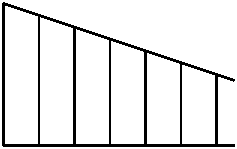
\includegraphics[width=0.22\textwidth]{gesamttex/edit_VIII-4/images/LH_37_04_156-3_d_156r.pdf}
\edcaption%
{\lbrack \textit{Fig.\:1}\rbrack}%
\end{edfigure}%
\selectlanguage{latin}%
\frenchspacing%
\normalsize%
